\section{Aufbau}
\label{sec:Aufbau}

\begin{figure}[H]
         \centering
         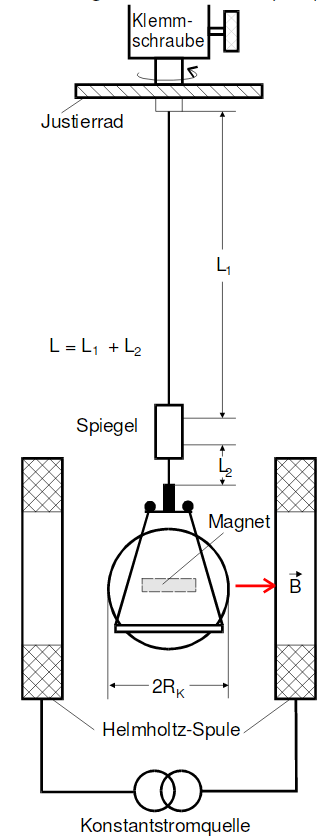
\includegraphics[width=\linewidth-150pt,height=\textheight-150pt,keepaspectratio]{content/Bilder/Aufbau.png}
         \caption{Messapperatur zur Bestimmung des Schubmoduls $G$ und des magnetischen Moments $m$ \cite{V102}.}
         \label{fig:Aufbau}
       \end{figure}

        Ein Draht des zu betrachtenden Materials wird oben mit einer Klemmschraube fixiert. Mithilfe eines
           Justierrades lässt er sich dann nurnoch drehen. Zur Besseren
            Betrachtung der auftretenden Drehschwingung wird ein Spiegel nach einer Länge $L_1$ eingesetzt. Der
             Spiegel wird über ein weiteres, kürzeres Stück Draht der Länge $L_2$ mit
             einer Haltekonstruktion verbunden, in welcher sich die bereits
              beschriebene Kugel befindet.
               Um die auftretende Schwingung zu dämpfen ist eine Dämpfkonstruktion
                unter der Kugelhalterung angebracht. Zur Vereinfachung der späteren Messung des magnetischen Moments ist ein Stabmagnet
               bereits in die Kugel integriert und ein Helmholtzspulenpaar um die Kugel aufgestellt. Dieses wird
                 mit einer Konstantstromquelle betrieben.

                 Nun zur genaueren Betrachtung der Zeitmessung mithilfe des Drehspiegels:

                 \begin{figure}[H]
                          \centering
                          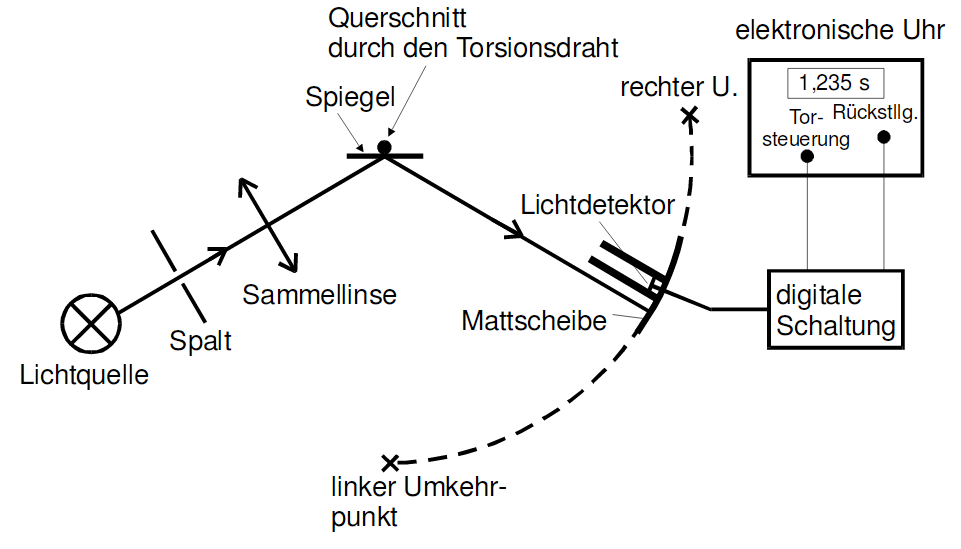
\includegraphics[width=\linewidth-150pt,height=\textheight-150pt,keepaspectratio]{content/Bilder/Drehspiegel.png}
                          \caption{Aufbau zur genauen Bestimmung der Periodendauer mithilfe eines Drehspiegels \cite{V102}.}
                          \label{fig:Drehspiegel}
                        \end{figure}
Zur besseren Betrachtung des Drehwinkels $\varphi$ wird das Licht einer Glühbirne
 mithilfe eines Spaltes und einer Sammellinse fokussiert und so ausgerichtet,
  dass es auf den Drehspiegel trifft. Während $\varphi$ sich ändert fährt der
   Lichtstrahl einen Pfad mit zwei Umkehrpunkten ab. Auf diesem Pfad ist eine
    Photodiode montiert, welche ein Signal abgibt, wenn der Lichtstrahl
     diese überstreicht. Die Impulse werden über eine digitale Schaltung verarbeitet und
      gelangen zu einer elektronischen Uhr, mit welcher schließlich die Periodendauer $T$ gemessen wird.

      Die digitale Schaltung ist wie folgt aufgebaut:
      \begin{figure}[H]
               \centering
               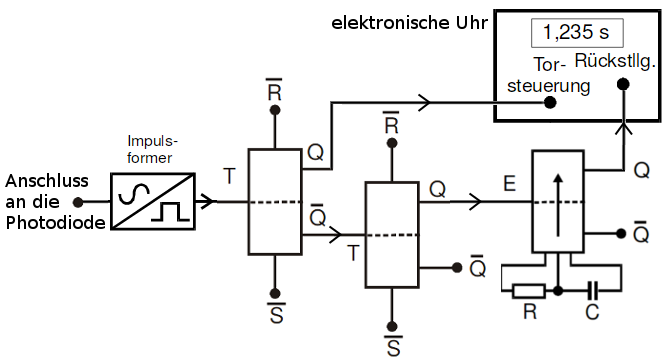
\includegraphics[width=\linewidth-150pt,height=\textheight-150pt,keepaspectratio]{content/Bilder/Digimist.png}
               \caption{Aufbau der digitalen Schaltung zum starten, stoppen und zurücksetzen der elektronischen Uhr \cite{V102}\cite{V104}.}
               \label{fig:digimist}
             \end{figure}
             An den Ausgängen Q können zwei Potentiale auftreten H und L. An $\overline{\text{Q}}$ liegt das jeweils andere Potential vor. Das Potential am Ausgang Q der bistabilen Kippstufen ändert sich bei einem Übergang am Eingang T vom Potential H zu L. Bei der monostabilen Kippstufe ändert sich das Potential am Ausgang Q, beim Übergang von T zu H am Eingang E, auf H. Nach einer kurzen Zeit ändert sich das Potential am Ausgang Q wieder zurück auf L. Die elektronische Uhr schaltet immer bei einem Übergang von H nach L.
              
             Über den Anschluss an die Photodiode gelangt jedes mal ein Nadelimpuls in den Impulsformer, wenn der Lichtstrahl über die Photodiode streicht. Dort wird dieser in einen Rechteckimpuls umgewandelt. Zu Beginn, bevor der Lichtstrahl das erste Mal die Photodiode überstrichen hat, ist das Potential an den Ausgängen Q das Potential L. Überstreicht der Lichtstrahl nun das erste Mal die Photodiode, so ändern sich die Potentiale an der ersten bistabilen Kippstufe. Die elektronische Uhr wird nicht gestartet. Auch an der zweiten bistabilen Kippstufe ändern sich die Potentiale. Dadurch ändert sich das Potential an der monostabilen Kippstufe und die Uhr wird zurückgesetzt. Bei dem zweitem Mal, dass der Lichtstrahl die Photodiode überstreicht ändern sich wieder die Potentiale an der ersten bistabilen Kippstufe. Nun startet die Uhr, da am Ausgang Q ein Übergang vom Potential H nach L stattfindet. Die anderen Potentiale ändern sich nicht. Bei dem drittem Mal ändern sich wieder die Potentiale an der ersten und zweiten bistabilen Kippstufe. Wenn der Lichtstrahl zum vierten Mal die Photodiode überstreicht ändert sich die Potentiale an den Ausgängen der ersten bistabilen Kippstufe und die Uhr wird wieder gestoppt. Nun befindet sich das System wieder im ursprünglichem Zustand.
             
             Die Schaltung in Abbildung 3 startet also beim 2. eingehenden Impuls die Zeitmessung und stoppt diese nach dem 4. Impuls wieder. Die gemessene Zeit wird nach dem 5. Impuls zurückgesetzt und nach dem 6. Impuls beginnt die nächste Messung. Da die vergangene Zeit zwischen dem ersten und letzten von drei eingehenden Impulsen gemessen werden sollte, erfüllt die Schaltung in Abbildung 3 die gewünschte Funktion.
